\documentclass[addpoints,answers,a4paper,11pt]{exam}
\usepackage{amssymb,amsmath}
\usepackage[usenames]{color}
\usepackage{multicol,fancybox,tabularx,textcomp,tabulary,pbox,ifthen}
\usepackage[dvipsnames]{xcolor}
\usepackage{blkarray}
\usepackage{booktabs}
\usepackage{multirow}
\usepackage{multicol}
\usepackage{makecell}
\usepackage{tikz}

%***************** solutions color etc preferences ********************
\unframedsolutions
%\shadedsolutions
%\definecolor{SolutionColor}{rgb}{.98,.98,.98}
%\renewcommand{\solutiontitle}{\noindent\textsf{Soln.:}\par\noindent}

%******************** Course Details *********************************
\newcommand{\testname}{End-Semester Examination}
\newcommand{\courseno}{MA 324}
\newcommand{\coursename}{Statistical Inference and Multivariate Analysis}
\newcommand{\instiname}{IIT GUWAHATI}
\newcommand{\testdate}{May 8, 2026}
\newcommand{\testtime}{14:00--17:00 IST}
\newcommand{\semester}{2025-26 Even}

%*****************************************************************************
\newcommand{\emptyframedbox}{\framebox{\rule{0pt}{10pt}{\rule{10pt}{0pt}}}}
\newcommand{\emptyrollno}{\emptyframedbox\emptyframedbox\emptyframedbox\emptyframedbox\emptyframedbox\emptyframedbox\emptyframedbox\emptyframedbox\emptyframedbox}
\newcommand{\emptyname}{\emptyframedbox\emptyframedbox\emptyframedbox\emptyframedbox\emptyframedbox\emptyframedbox\emptyframedbox\emptyframedbox\emptyframedbox\emptyframedbox\emptyframedbox\emptyframedbox\emptyframedbox\emptyframedbox\emptyframedbox\emptyframedbox\emptyframedbox\emptyframedbox\emptyframedbox}

%************* FOR FOOTER AND HEADER **********************************
% page foot and header
\pagestyle{headandfoot}

\firstpagefooter{}{}{\tiny Page \thepage\ of \numpages\normalsize}
\runningheader{\semester}{\testname}{\courseno}
\runningheadrule
%\runningfootrule
\runningfooter{}{}{\tiny Page \thepage\ of \numpages\normalsize}
%****************** TO REDUCE MARGINS*******************
\extrawidth{.65in}
\extraheadheight{-0.25in}
\extrafootheight{-0.40in}
%**END--OF--PROOF: stretch is a rubber space which fills. * ensures it works at beginning of line
\newcommand{\eop}{\hspace*{\stretch{1}}{\scriptsize\maltese}}
\renewcommand{\eop}{}
%stretch is a rubber space which fills. * ensures it works at beginning of line
\newcommand{\push}{\hspace*{\stretch{1}}}
%to separate advanced questions
%\newcommand{\advanced}{\fullwidth{\raisebox{-2pt}{$\ll$}{\hrulefill}\raisebox{-2pt}{\tiny\fbox{ADVANCED}}{\hrulefill}\raisebox{-2pt}{$\gg$}}}
\newcommand{\advanced}{\fullwidth{\hrulefill\raisebox{-2pt}{\tiny\fbox{ADVANCED}}\hrulefill}}
%ignore extra spaces around enviroments
%\ignorespaces
\parindent 0pt
%**********some exam package options
%\usehorizontalhalf
%\marginpointname{}
%\marginbonuspointname{}
%\pointsinmargin
%\pointformat{[\themarginpoints $^\mathrm{pnts.}$]}
%\bonuspointformat{[\themarginpoints $^\mathrm{xtra}$]}

% %*********** step mark macro *************************
% \newif\ifstepmark
% \newcommand{\stepmark}[1]{\ifstepmark
%       \,\,\colorbox{Green!40!}{[{#1}\,point\ifdim#1pt=1pt%
%          \else
%             s
%          \fi%
%       ]}
%    \else%
%       {}
%    \fi%
% }

\newcommand{\blankpages}[1]{
   \ifthenelse{\boolean{printanswers}}
   {}
   {
      \foreach \n [count=\ni] in {1,...,#1}{%
         \ifnum\ni=#1% 
            \newpage%
         \else%
            \newpage%
            \mbox{}%
         \fi%
      }
   }
}

\printanswers
%\stepmarktrue
%\stepmarkfalse

\begin{document}

\textsc{{\normalsize\courseno \push \testname}\smallskip\\
{\normalsize\coursename \push \testtime}\smallskip\\
{\normalsize\instiname \push \testdate}}
\begin{center}
   \fbox{\large{\textsc{\textbf{PART-B}}}}
\end{center}

\ifthenelse{\boolean{printanswers}}
{
   \fullwidth{\hrulefill\raisebox{-2pt}{\fbox{\textsc{Model Answers of
               \testname\ (Total points: \numpoints)}}}\hrulefill}
}
{
   \hrulefill\\[5mm]
   Name of the Student: \hrulefill\\[5mm]
   Signature of the Student: \hrulefill \hspace{10mm} Roll No.: \hrulefill\\[5mm]
   Signature of the Invigilator: \hrulefill
   \fullwidth{\hrulefill\raisebox{-2pt}{\footnotesize\fbox{\textsc{Instructions}}}\hrulefill}
   \begin{enumerate}
      % \item To `print' means to write legibly in capital letters.
      % \item Put your signature in the space provided:$\rightarrow$ \push
      % \framebox{\rule{100pt}{0pt}\rule{0pt}{10pt}} 
      % \item Print your roll number:$\rightarrow$ \push \emptyrollno
      % \item Print your name as registered:\push \emptyname
      \item Check that you have \textbf{\numpages\  printed pages}. The PART-B
         of the examination has \textbf{\numquestions\ questions}, for a total of
         \textbf{\numpoints\ points}.
      \item Attempt \textbf{all questions}.
      \item There is \textbf{no credit} for a solution if the appropriate work is not
         shown, even if the answer is correct.
      \item Write your answers in this booklet and only in the \textbf{space marked for
         answers}. Any answer written in any space other than the designated space will
         \textbf{not be evaluated}.
      \item The pages numbered \textbf{8 to 10} are kept as \textbf{additional pages}. If
         you cannot able to fit a complete answer in the space provided just
         after the question, you can use these three pages by referring the page
         number of additional page in the original space.
      \item At the beginning of the examination, a supplementary sheet has been
         provided only for rough work. Should you need more, please ask the
         invigilator.
      \item No questions require any clarification from the instructor or
         invigilators, even if a question has an error or incomplete data. The
         students are advised to write answer according to their understanding
         or write reasons for why it is not possible to solve partially or
         completely that question by citing errors/insufficient data. 
   \end{enumerate}

   \fullwidth{\hrulefill\raisebox{-2pt}{\footnotesize\fbox{\textsc{For Office Use Only}}}\hrulefill}

   \vspace{0.2in}
   \begin{center}
      \cellwidth{12mm} 
      \gradetablestretch{3.0}
      \gradetable[h][questions]
   \end{center}

   \newpage

   \fullwidth{\hrulefill\raisebox{-2pt}{\footnotesize\fbox{\textsc{Questions}}}\hrulefill}
}

\begin{questions}

   \question[6]
   Let 
   \begin{align*}
      \boldsymbol{S} &= \begin{pmatrix} 
         S_{yy} & S_{y \boldsymbol{X}}^{\,\textcolor{red}{T}} \\
         S_{y \boldsymbol{X}} & S_{\boldsymbol{X} \boldsymbol{X}}
      \end{pmatrix}      
   \end{align*}
   be the partitioned sample covariance matrix of $Y_{1\times 1}$ and
   $\boldsymbol{X}_{q \times 1}$ based on a centered (with respect to sample
   mean) sample of size $n$.  Prove that the squared sample first canonical
   correlation $r_1^2$ is identical to the coefficient of determination ($R^2$)
   obtained from the multiple linear regression of $Y$ on the vector
   $\boldsymbol{X}$.

   \begin{solution}
      In standard CCA, the squared sample canonical correlations are
      the eigenvalues of the matrix 
      \begin{align*}
         \mathbf{S}_{11}^{-\frac{1}{2}}
         \mathbf{S}_{12} \mathbf{S}_{22}^{-1}
         \mathbf{S}_{21}\mathbf{S}_{11}^{-\frac{1}{2}} = 
         \frac{1}{s_{yy}} \mathbf{s}_{yX}^T
         \mathbf{S}_{XX}^{-1} \mathbf{s}_{Xy}.
      \end{align*}
      Notice that $\mathbf{s}_{yX}^T$ is a $1 \times q$ vector,
      $\mathbf{S}_{XX}^{-1}$ is a $q \times q$ matrix, and $\mathbf{s}_{Xy}$
      is a $q \times 1$ vector. The resulting product is a $1 \times 1$
      scalar. The only eigenvalue of a scalar is the scalar itself.
      Therefore, the single squared canonical correlation is
      \begin{equation} \label{eq:r2}
         r_1^2 = \frac{\mathbf{s}_{yX}^T \mathbf{S}_{XX}^{-1}
         \mathbf{s}_{Xy}}{s_{yy}}.
      \end{equation}

      Now, consider the multiple linear regression of $Y$ on
      $\mathbf{X}$. The estimated regression coefficient vector is given by
      the standard ordinary least squares (OLS) solution:
      \begin{equation*}
         \hat{\boldsymbol{\beta}} = \mathbf{S}_{XX}^{-1} \mathbf{s}_{Xy}
      \end{equation*}
      % The portion of the variance in $Y$ explained by the regression model
      % (the Explained Variance) is calculated as $\hat{\boldsymbol{\beta}}^T
      % \mathbf{s}_{Xy}$:
      Therefore,
      \begin{align*}
         SS_{Reg} &= \widehat{\boldsymbol{\beta}}^{T} S_{yX} = (\mathbf{S}_{XX}^{-1} \mathbf{s}_{Xy})^T \mathbf{s}_{Xy}
         = \mathbf{s}_{yX}^T (\mathbf{S}_{XX}^{-1})^T \mathbf{s}_{Xy}
         = \mathbf{s}_{yX}^T \mathbf{S}_{XX}^{-1} \mathbf{s}_{Xy},
      \end{align*}
      since $(\mathbf{S}_{XX}^{-1})^T = \mathbf{S}_{XX}^{-1}$.  Therefore,
      \begin{equation} \label{eq:R2}
         R^2 = \frac{SS_{Reg}}{SS_T} =
         \frac{\mathbf{s}_{yX}^T \mathbf{S}_{XX}^{-1}
      \mathbf{s}_{Xy}}{s_{yy}}.
      \end{equation}
      By comparing equations (\ref{eq:r2}) and (\ref{eq:R2}), we have $r_1^2 = R^2$.
   \end{solution}

   \blankpages{2}

   \question
   Suppose you are performing a factor analysis on a $4 \times 4$ sample
   covariance matrix $\mathbf{S}$. The eigenvalues of $\mathbf{S}$ are
   $\lambda_1 = 0.8$, $\lambda_2 = 2.1$, $\lambda_3 = 4.2$, and $\lambda_4 =
   0.2$. The corresponding normalized eigenvectors are $\mathbf{e}_1,
   \mathbf{e}_2, \mathbf{e}_3,$ and $\mathbf{e}_4$. You decide to extract $m=2$
   factors using the principal component method.

   \begin{parts}
      \part[2] Write down the explicit mathematical expression for the estimated
      factor loading matrix $\tilde{\mathbf{L}}$ in terms of the given
      eigenvalues and eigenvectors.
      \begin{solution}
         In the principal component method of factor analysis, the columns of
         the estimated factor loading matrix $\tilde{\mathbf{L}}$ are derived
         as follows: Frist, the eigenvalues are arranged in descending order of
         magnitude. Then, the largest $m$ eigenvalues and corresponding
         normalized normalized eigenvectors by the square root of
         their corresponding eigenvalues. \\
         Since $m=2$, the $4 \times 2$ matrix $\tilde{\mathbf{L}}$ is given by:
         \begin{equation*}
            \tilde{\mathbf{L}} = \begin{bmatrix} \sqrt{\lambda_3} \mathbf{e}_3 &
            \sqrt{\lambda_2} \mathbf{e}_2 \end{bmatrix} .
            \end{equation*}
         \end{solution}

         \part[1] Let the first row of $\tilde{\mathbf{L}}$ be $\tilde{\mathbf{l}}_1^T
         = [0.8, -0.4]$. Calculate the estimated communality $\tilde{h}_1^2$ for
         the first variable.
         \begin{solution}
            The estimated communality for the $i$-th variable, $\tilde{h}_i^2$,
            represents the portion of the variable's variance explained by the $m$
            common factors. It is calculated as the sum of squared loadings for
            that variable (i.e., the squared Euclidean norm of the $i$-th row of
            $\tilde{\mathbf{L}}$).
            \begin{align*}
               \tilde{h}_1^2 &= \tilde{l}_{11}^2 + \tilde{l}_{12}^2 \implies
               \tilde{h}_1^2 = (0.8)^2 + (-0.4)^2 = 0.8.
            \end{align*}
         \end{solution}

         \part[4] Prove that the sum of all estimated communalities $\sum_{i=1}^p
         \tilde{h}_i^2$ is exactly equal to the sum of the largest $m=2$
         eigenvalues of $\mathbf{S}$.
         \begin{solution}
            Let $\tilde{l}_{ij}$ be the element in the $i$-th row and $j$-th column
            of $\tilde{\mathbf{L}}$. The sum of all estimated communalities is:
            \begin{equation*}
               \sum_{i=1}^p \tilde{h}_i^2 = \sum_{i=1}^p \left( \sum_{j=1}^m
               \tilde{l}_{ij}^2 \right).
            \end{equation*}
            By interchanging the order of summation, we get:
            \begin{equation*}
               \sum_{i=1}^p \tilde{h}_i^2 = \sum_{j=1}^m \left( \sum_{i=1}^p
               \tilde{l}_{ij}^2 \right).
            \end{equation*}
            The inner sum $\sum_{i=1}^p \tilde{l}_{ij}^2$ is the sum of squared
            elements in the $j$-th column of $\tilde{\mathbf{L}}$. From Part (a),
            the $j$-th column is $\sqrt{\lambda_j} \mathbf{e}_j$. The squared norm
            of this column is:
            \begin{equation*}
               (\sqrt{\lambda_j} \mathbf{e}_j)^T (\sqrt{\lambda_j} \mathbf{e}_j) =
               \lambda_j (\mathbf{e}_j^T \mathbf{e}_j) .
            \end{equation*}
            Because the eigenvectors are normalized (orthonormal), $\mathbf{e}_j^T
            \mathbf{e}_j = 1$. Therefore, the inner sum equals $\lambda_j$.
            Substituting this back yields:
            \begin{equation*}
               \sum_{i=1}^p \tilde{h}_i^2 = \sum_{j=1}^m \lambda_j .
            \end{equation*}
      \end{solution}

      % \part[2] If we had used the sample correlation matrix $\mathbf{R}$ instead of
      % $\mathbf{S}$, what is the maximum possible value for any single estimated
      % communality $\tilde{h}_i^2$? Justify your answer.
      % \begin{solution}
      %    If the sample correlation matrix $\mathbf{R}$ is used, the variance of
      %    every standardized variable is exactly $1$ (the diagonal elements of
      %    $\mathbf{R}$ are $r_{ii} = 1$). 
      %
      %    By definition in the orthogonal factor model, the variance of the
      %    $i$-th variable is partitioned into communality and specific variance:
      %    \begin{equation*}
      %       Var(Z_i) = \tilde{h}_i^2 + \tilde{\psi}_i = 1
      %    \end{equation*}
      %    Because specific variance $\tilde{\psi}_i$ must be non-negative
      %    ($\tilde{\psi}_i \ge 0$), it mathematically follows that:
      %    \begin{equation*}
      %       \tilde{h}_i^2 \le 1
      %    \end{equation*}
      %    Therefore, the maximum possible value for any estimated communality
      %    $\tilde{h}_i^2$ is \textbf{1}. \\
      %    \textit{(Award points for explicitly referencing that diagonals of
      %    $\mathbf{R}$ are 1 and that specific variances cannot be negative.)}
      % \end{solution}
   \end{parts}

   \blankpages{2}

   \question[5]
   Let $X_1, X_2, \dots, X_n$ be a random sample of size $n$ from a distribution
   with mean $\mu \in \mathbb{R}$ and variance $\mu^2$. Let $\overline{X}_n =
   \frac{1}{n}\sum_{i=1}^{n} X_i$. Derive a variance-stabilizing transformation
   $g(\overline{X}_n)$ such that the asymptotic variance of $g(\overline{X}_n)$
   does not depend on $\mu$. 

   \begin{solution}
      Using CLT, we have
      \begin{align*}
         \sqrt{n} (\bar{X}_n - \mu) &\xrightarrow{d} Z_1 \sim N(0, c\mu^2).
      \end{align*}
      Using delta method,
      \begin{align*}
         \sqrt{n} (g(\bar{X}_n) - g(\mu)) &\xrightarrow{d} Z_2 \sim N(0, c\mu^2(g'(\mu))^2).
      \end{align*}
      Thus, we want $g(\cdot)$ such that
      \begin{align*}
         \mu^2(g'(\mu))^2 &= k \quad (\text{some constant } k).
      \end{align*}
      Therefore, a variance-stabilizing transformation satisfies
      \begin{align*}
         g'(\mu) &= \frac{1}{\mu} \implies g(\mu) = \ln \mu.
      \end{align*}
      Thus, $g(x) = \ln x$ is a variance-stabilizing transformation.
   \end{solution}

   \blankpages{1}

   \question[2]
   The figure below displays a Normal Q-Q plot for a dataset of size $n = 50$.
   Interpret this plot to determine if the data follows a normal distribution.
   If the normality assumption is violated, specify which class of distributions
   would more accurately characterize the data.
   \begin{center}
      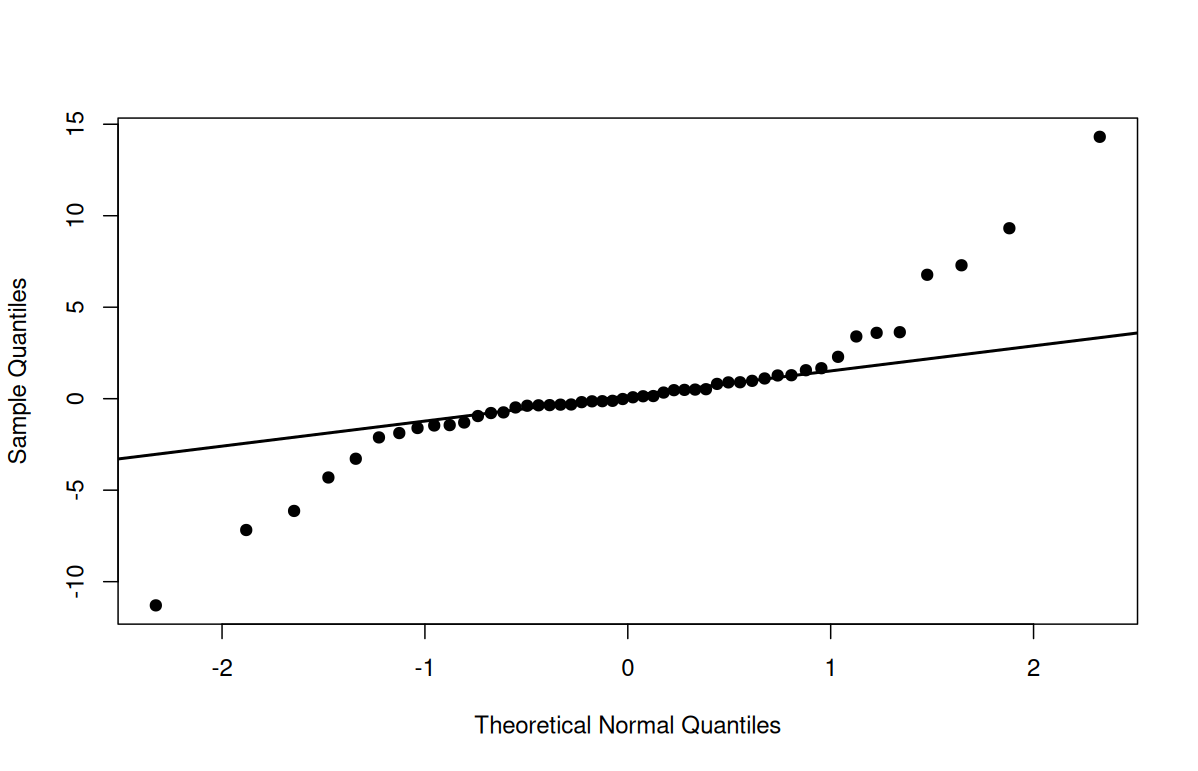
\includegraphics[width=0.8\textwidth]{QQplot.png}
   \end{center}

   \begin{solution}
      The S-shaped curvature indicates that the distribution has heavier tails
      than a normal distribution. Therefore, a normal distribution will not give
      a good fit and a heavy tailed distribution would provide better fit to the
      model.

      \textbf{Note:} 
      \begin{enumerate}
         \item About half of the observed values are negative. Therefore, a
            distribution with support in $[0,\,\infty)$ is not a plausible
            distribution. 
         \item Looking in to the given plot, it is difficulty to say exactly
            which distribution will provide a good fit among heavy tailed
            distributions. For that you need to draw Q-Q plot or that
            distribution.
      \end{enumerate}
   \end{solution}
   
   \blankpages{1}

   \ifthenelse{\boolean{printanswers}}
   {
   }
   {
      \fullwidth{\hrulefill\raisebox{-2pt}{\footnotesize\fbox{\textsc{Additional
      Pages for Answers}}}\hrulefill}
   }

   \blankpages{3}

\end{questions}

\end{document}
